\section{平面图}

\subsection{基本定义}

\begin{frame}{平面图定义}
若图G可画在平面上，使得任意两条边都不会在非端点处相交，则称G是平面图。
\end{frame}

\subsection{欧拉定理}
\begin{frame}{欧拉定理}
欧拉定理建立了平面图中点数、边数和域数的关系，可以知二求一。 \newline \newline

对于平面图，如果有F个面，E条边，V个点，k个连通块，那么有公式

$F=E-V+k+1$

证明：使用归纳法。当$E=0$时，$k=V$，等式成立。然后一条一条加边，如果加入边的两个点未联通，则$k--,E++$，等式不变。如果加入的两个点已联通，则这条边必然把某个域一分为二，等式两边同时$+1$，得证。
\end{frame}

\begin{frame}{性质}
\begin{itemize}
    \item $E \le 3n-6$
        \begin{proof}
            每个域至少有三条边，每条边最多与两个域相连，所以$F \le \frac{2}{3}E$

            那么$E-V+k+1 \le \frac{2}{3}E$，同时有$k \ge 1$，所以$E \le 3n-6$
        \end{proof}
    \item $k \le 2n-4$
        \begin{proof}
            把$F \le \frac{2}{3}E$的E用欧拉公式代换得

            $\frac{3}{2}F \le F+V-k-1 \rightarrow F \le 2V-2k-2$,同时有$k \ge 1$,得证
        \end{proof}
\end{itemize}
\end{frame}

\begin{frame}{P3776 [APIO2017] 斑斓之地}
    题目描述：一个 $r \times c$ 的方格表，一只蛇在上面爬导致部分方格表变成了河。多次询问，每次询问只保留某个矩形内的格子，问非河的部分形成了多少个连通块。
\end{frame}

\begin{frame}{P7295 [USACO21JAN] Paint by Letters P}
    考虑这样一个问题：给你一棵树，只考虑区间 \([l,r]\) 中的点，形成几个连通块（数量只需要求为 \(\leq i < j \leq r\) 且 \((i,j) \in E\) 的 \((i,j)\) 数量（可以认为是边点之类的东西）。

    一般平面图也可以套用这个做法。本题中在相邻非网格子之间连边，那么只需要反映：点数、面数和边数。

    点数容易，那么真难则反扫描线以下即可（如果强制在线，就主席树），边数几乎一样。

    考虑可能出现什么样的“面”。首先所有 \(2 \times 2\) 的矩形一定是他的，还有没有其他的？

    蛇的形态非常关键——所有河都是连通的。因此，还有另一种环——包裹了整条蛇的环，单独处理一下就行。
\end{frame}


\subsection{平面图与对偶图}

\begin{frame}{平面图对偶图定义}

\begin{multicols}{2}
    
对偶图：

原图的每个域成为新图的一个点

原图的每个点作为新图的一个域

\begin{center}
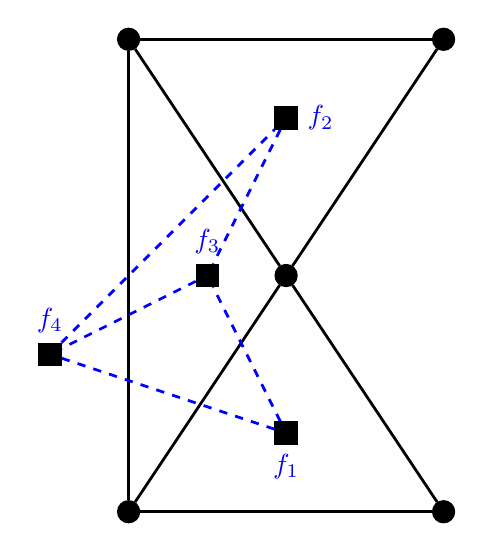
\begin{tikzpicture}[
    node distance=1.5cm,
    vertex/.style={circle, minimum size=8pt, draw, fill=black, inner sep=0pt},
    dual_vertex/.style={rectangle, draw, fill=black, minimum size=8pt, inner sep=0pt},
    edge/.style={line width=1pt},
    dual_edge/.style={line width=1pt, blue, dashed}
]

% 绘制平面图节点
\node[vertex] (v1) at (0,0) {};
\node[vertex] (v2) at (4,0) {};
\node[vertex] (v3) at (2,3) {};
\node[vertex] (v4) at (0,6) {};
\node[vertex] (v5) at (4,6) {};

% 绘制平面图边
\draw[edge] (v1) -- (v2);
\draw[edge] (v1) -- (v3);
\draw[edge] (v2) -- (v3);
\draw[edge] (v3) -- (v4);
\draw[edge] (v3) -- (v5);
\draw[edge] (v4) -- (v5);
\draw[edge] (v1) -- (v4);

% 绘制对偶图节点（面）
\node[dual_vertex] (f1) at (2,1) {};
\node[dual_vertex] (f2) at (2,5) {};
\node[dual_vertex] (f3) at (1,3) {};
\node[dual_vertex] (f4) at (-1,2) {};

% 绘制对偶图边
\draw[dual_edge] (f4) -- (f2);
\draw[dual_edge] (f1) -- (f3);
\draw[dual_edge] (f1) -- (f4);
\draw[dual_edge] (f2) -- (f3);
\draw[dual_edge] (f3) -- (f4);

% 标记对偶图节点
\node[blue, below] at (f1.south) {$f_1$};
\node[blue, right] at (f2.east) {$f_2$};
\node[blue, above] at (f3.north) {$f_3$};
\node[blue, above] at (f4.north) {$f_4$};

\end{tikzpicture}
\end{center}
\end{multicols}

\end{frame}

\begin{frame}{平面图转对偶图}{算法}
将每条边拆分成两条有向边，并将每个点出发的有向边按顺时针排序。

选择任意一条未访问的边出发，在每个节点处选择绕该点顺时针旋转遇到的第一条边为下一条边，直到回到初始边。这样就走完的一个域周围的边。不断重复，直到所有边均被走过。

为每个域建立一个点。如果一条无向边被两个域共用，那么在这两个域之间连上这条边
\end{frame}

\begin{frame}
\frametitle{对偶图的应用}
\begin{multicols}{2}
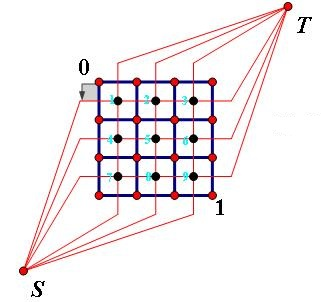
\includegraphics[width=5cm]{geometry/duioutu.jpg}

\begin{center}
平面图最大流
\begin{displaymath}
    \Downarrow
\end{displaymath}

平面图最小割
\begin{displaymath}
    \Downarrow
\end{displaymath}
对偶图最短路
\end{center}
\end{multicols}
\end{frame}

\begin{frame}{P4001 ICPC-Beijing 2006 狼抓兔子}

\begin{minipage}{0.4\textwidth}
    
给定这样一张网格图：左上角点为 $(1,1)$，右下角点为 $(N,M)$（图中 $N=3$，$M=4$）。有以下三种类型的道路：

1. $(x,y)\rightleftharpoons(x+1,y)$

2. $(x,y)\rightleftharpoons(x,y+1)$

3. $(x,y)\rightleftharpoons(x+1,y+1)$
\end{minipage}
\hfill % 两列之间的间距
\begin{minipage}{0.58\textwidth}
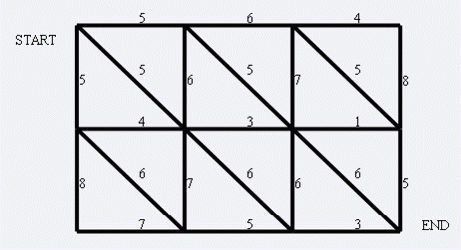
\includegraphics[width=\textwidth]{geometry/planar.png}
\end{minipage}


道路上的权值表示这条路上最多能够通过的兔子数，道路是无向的。左上角和右下角为兔子的两个窝，开始时所有的兔子都聚集在左上角 $(1,1)$ 的窝里，现在它们要跑到右下角 $(N,M)$ 的窝中去，狼王开始伏击这些兔子。当然为了保险起见，如果一条道路上最多通过的兔子数为 $K$，狼王需要安排同样数量的 $K$ 只狼，才能完全封锁这条道路，你需要帮助狼王安排一个伏击方案，使得在将兔子一网打尽的前提下，参与的狼的数量要最小。($N,M \le 1000$)
\end{frame}

\begin{frame}{P2046 [NOI2010] 海拔}
    YT 市是一个规划良好的城市，城市被东西向和南北向的主干道划分为 $n \times n$ 个区域。简单起见，可以将 YT 市看作 一个正方形，每一个区域也可看作一个正方形。从而，YT 城市中包括 $(n+1) \times (n+1)$ 个交叉路口和 $2n \times (n+1)$ 条双向道路（简称道路），每条双向道路连接主干道上两个相邻的交叉路口。下图为一张 YT 市的地图（$n = 2$），城市被划分为 $2 \times 2$ 个区域，包括 $3 \times 3$ 个交叉路口和 $12$ 条双向道路。

    小 Z 作为该市的市长，他根据统计信息得到了每天上班高峰期间 YT 市每条道路两个方向的人流量，即在高峰期间沿着该方向通过这条道路的人数。每一个交叉路口都有不同的海拔高度值，YT 市市民认为爬坡是一件非常累的事情，每向上爬 $h$ 的高度，就需要消耗 $h$ 的体力。如果是下坡的话，则不需要耗费体力。因此如果一段道路的终点海拔减去起点海拔的值为 $h$（注意 $h$ 可能是负数），那么一个人经过这段路所消耗的体力是 $\max\{0, h\}$。

    小 Z 还测量得到这个城市西北角的交叉路口海拔为 $0$，东南角的交叉路口海拔为 $1$（如上图所示），但其它交叉路口的海拔高度都无法得知。小 Z 想知道在最理想的情况下（即你可以任意假设其他路口的海拔高度），每天上班高峰期间所有人爬坡消耗的总体力和的最小值。
\end{frame}

\begin{frame}{P10665 [AMPPZ2013] Bytehattan}
\end{frame}

\begin{frame}{P4646 [IOI 2007] flood 洪水}
\end{frame}

\begin{frame}{P7916 [CSP-S 2021] 交通规划}
\end{frame}

\begin{frame}{CF750H. New Year and Snowy Grid}
    有一张有障碍的$h \times w$的网格图，问是否存在一条路径，从左上角出发到右下角，再回到左上角，且不会重复经过同一个点（起点除外）。
    
    有$q$组询问，每组询问给出$k$个非障碍点，问是否存在不经过这$k$个点的合法路径。

    $h,w \le 10^3，q \le 10^4，k \le 10$
\end{frame}

\begin{frame}{CF750H. New Year and Snowy Grid}
    \begin{itemize}
        \item 首先，问题相当于求起点到终点是否存在两条不相交的路径。
        \item 如果只有一组询问的话，那就是一个经典的网络流模型，我们可以给每个点拆点，如果这个点是障碍点，那么$i$向$i'$连流量为$0$的边，否则，$i$向$i'$连流量为$1$的边，表示每个点只能经过一次。再每个点向其周围的$4$个点连流量为$1$的边。
        \item 然后从$S$到$T$跑一边最大流，如果流量小于$2$，那么答案就是NO，否则就是YES。
        \item 接着我们可以把最大流问题转换成最小割问题，不过遗憾的是之前的建图并不是平面图，不能转换成最短路问题。
    \end{itemize}
\end{frame}

\begin{frame}{CF750H. New Year and Snowy Grid}
    \begin{itemize}
        \item 我们可以用一个巧妙的办法，直接考虑最短路模型，S向所有$(i,1)(2 \le i \le n)$和$(n,j)(1 \le j<m)$连边，也就是最左边的那一列和最下边的那一行。所有$(i,m)(1 \le i<n)$和$(1,j)(2 \le j \le m)$向$T$连边，也就是最右边的那一列和最上边的那一行。
        \item 然后所有点向八联通方向连边，边没有边权，每个点有点权，障碍点的点权为0，空地的点权为1。
        \item 跑一遍最短路，如果最短路小于$2$，那么答案就是NO，否则就是YES。
        \item 这样的复杂度就是最短路的复杂度了，考虑到点权只有$0$和$1$，我们可以bfs，于是，做一遍复杂度与图的边数有关，即$O(8nm)$的。
    \end{itemize}
\end{frame}

\begin{frame}{CF750H. New Year and Snowy Grid}
    \begin{itemize}
        \item 当然，继续观察可以发现，由于只要判断最短路与2的大小关系，所以问题就转化成：是否添加一个障碍物就可以使S到T的最短路为0，也就是，是否可以添加一个障碍物使得$S$和$T$联通。
        \item 关于联通性，很容易想到用并查集维护。
        \item 于是我们可以预处理出所有的障碍物形成的连通块，并预处理出所有相距为1的连通块对。
        \item 每次询问，把$k$个点周围的点用并查集连起来，最后看一下，所有与S并起来的连通块和所有与T并起来的连通块，是否存在连通块对相距为1，以及是否有新添的障碍点，满足这个点到S集的距离加上这个点到T集的距离不超过1。
    \end{itemize}
\end{frame}

\begin{frame}{平面图点定位}
\begin{multicols}{2}
平面图点定位求的是对于平面图中的一个点，它位于对偶图中的哪个域。

直接求解二维问题比较麻烦，我们的简化方法是把它进行梯形剖分。

基本假设：所有点横坐标互异(可以把所有点的x坐标随机扰动eps范围，保证没有相同横坐标)

在这个结构中，每个域均是梯形(三角形可看做是退化的梯形)。且域数仍然为O(n) \newline \newline

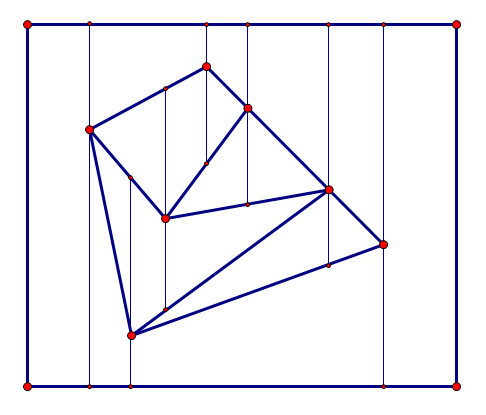
\includegraphics[width=5cm]{geometry/place.png}
\end{multicols}
\end{frame}
\begin{frame}
\frametitle{平面图点定位}
\begin{proof}
证明：每个点引出两条射线，至多增加两个节点。故节点总数不超过3*n。除节点处无交点，仍然是平面图。故域的数量仍是O(n)。
\end{proof}

如何构建这样一张平面图呢？我们用扫描线来完成。

把所有x坐标离散化，那么$x_{i-1} \ldots x_i$这段区间内的域和$x_i \ldots x_{i+1}$这段域的区别就在于有一些域在$x_i$结尾，应当删除，有一些域在$x_i$开头，应当加入。

然后注意到，$x_i \ldots x_{i+1}$这段区间内的所有域在纵坐标上是有严格的大小关系的，我们可以按照大小关系存储这些域。这样查询一个点的位置只需要二分就可以了。需要支持删除与插入，可以用一棵平衡树来实现。

如果需要在线，可以把平衡树可持久化。
\end{frame}

\begin{frame}{P4073 [WC2013] 平面图}
\end{frame}

\begin{frame}{P3249 [HNOI2016] 矿区}
\end{frame}


\subsection{三角剖分与V图}

\begin{frame}{Delaunay三角剖分}

假设V是二维实数域上的有限点集，边e是由点集中的点作为端点构成的封闭线段，E为e的集合。那么该点集V的一个三角剖分T=(V,E)是一个平面图G。

该平面图满足条件：
\begin{enumerate}
    \item 除了端点，平面图中的边不包含点集中的任何点。
    \item 没有相交边。
\end{enumerate}

平面图中所有的面都是三角面，且所有三角面的合集是点集V的凸包。
\end{frame}

\begin{frame}
\frametitle{Delaunay三角剖分}

Delaunay三角剖分是一种特殊的三角剖分。\newline \newline

Delaunay边：假设E中的一条边e(两个端点为A,B),e若满足下列条件，则称之为Delaunay边：存在一个圆经过A,B两点，圆内(注意是圆内，圆上最多三点共圆)不含点集V中任何其他的点，这一特性又称空圆特性。
\newline \newline

Delaunay三角剖分：如果点集V的一个三角剖分T只包含Delaunay边，那么该三角剖分称为Delaunay三角剖分。
\end{frame}

\begin{frame}{分治法构造Delaunay三角剖分}

首先对点集按x坐标排序。如果点集内点的个数小于等于3，那么直接构造，否则将点集拆分成两个大小差不多的点集进行构造，最后合并两点集的Delaunay三角剖分。\newline \newline

接下来考虑如何合并。
\end{frame}

\begin{frame}{分治法构造Delaunay三角剖分}{步骤一}
首先，求解两个点集的凸包的最下方的正切线,并连接两端点。

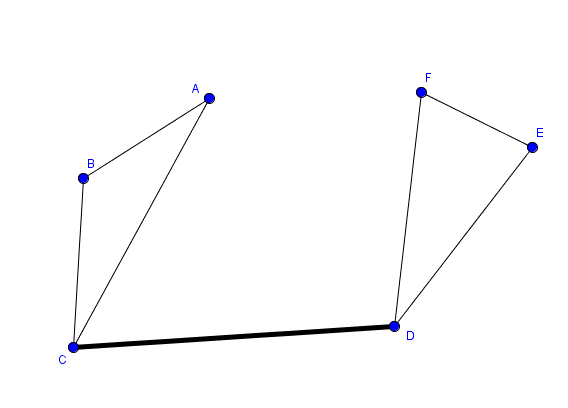
\includegraphics[height=5cm]{geometry/v1.png}
\end{frame}

\begin{frame}{分治法构造Delaunay三角剖分}{步骤二}
接下来，如图所示，CD为两个凸包的正切线，求出它们的中垂线$L_{CD}$。

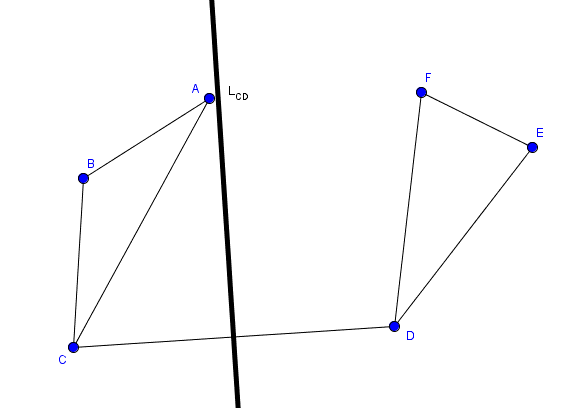
\includegraphics[height=5cm]{geometry/v2.png}
\end{frame}

\begin{frame}{分治法构造Delaunay三角剖分}{步骤三}
然后找到与C或D相连的边中，中垂线与$L_{CD}$有交点的边，如果有多个边，那么选择交点Y坐标最小的点所关联边。

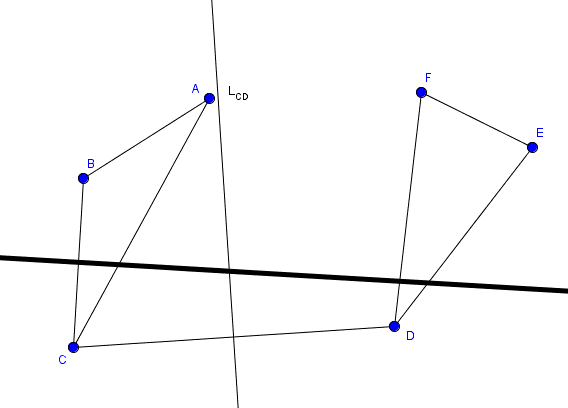
\includegraphics[height=5cm]{geometry/v3.png}
\end{frame}

\begin{frame}{分治法构造Delaunay三角剖分}{步骤四}
如图所示，选择的边为BC，那么连接BD，并且删除与BD相交的边。设BD为新产生的正切线。

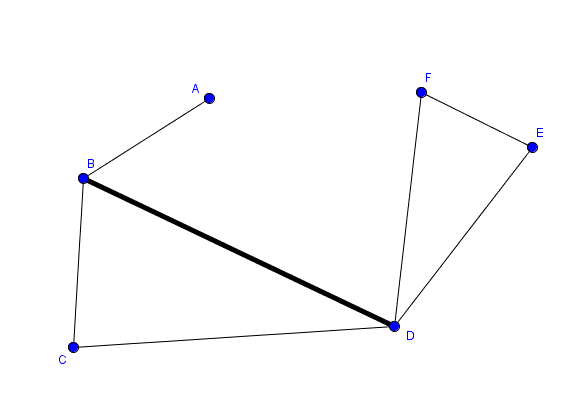
\includegraphics[height=5cm]{geometry/v4.png}
\end{frame}

\begin{frame}{分治法构造Delaunay三角剖分}{步骤五}
然后将BD像CD一样不断重复以上步骤，就可以合并两个点集的Delaunay三角剖分了。

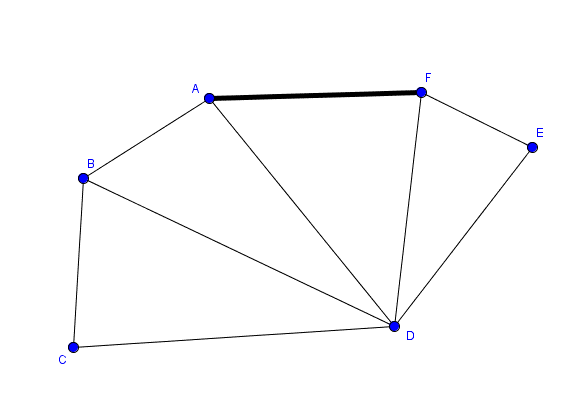
\includegraphics[height=5cm]{geometry/v5.png}
\end{frame}

\begin{frame}{分治法构造Delaunay三角剖分}{解释}

之前为什么选择交点纵坐标最小的边呢？

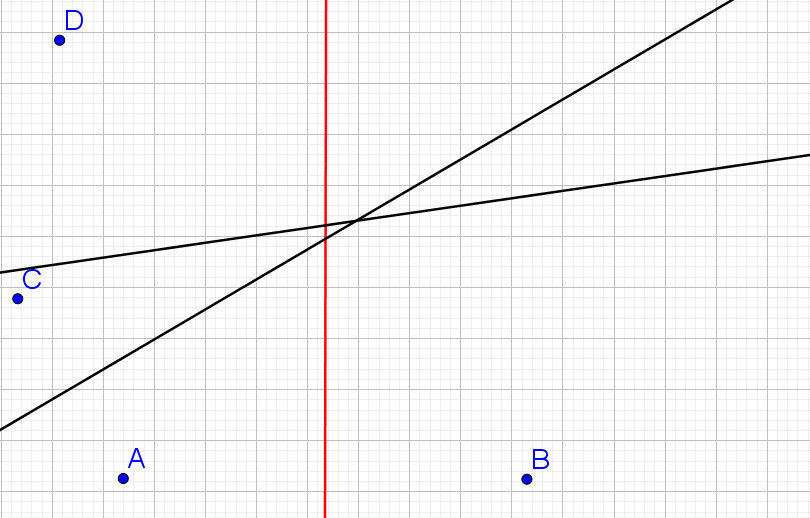
\includegraphics[height=2.5cm]{geometry/vgraph2.png}

考虑之前AC和AD都有边，AC的中垂线和AB的中垂线的交点在AD的中垂线和AB的中垂线的交点的下方。有一个结论：三个点两两的中垂线会相交于同一点，所以BC中垂线与AB的交点也会在BD中垂线与AB交点的下方。那
么BD中垂线就会被BC中垂线和BA中垂线完全覆盖，所以BD不能相邻。

把BC相连之后，如果存在D有AD与BC相交则AD的中垂线会被AC中垂线和AB中垂线覆盖，所以AD不能相邻。
\end{frame}

\begin{frame}{分治法构造Delaunay三角剖分}{优化}

分治法构建三角剖分的复杂度是期望nlogn的，但是可以被卡到平方以上。瓶颈在于上述操作3中，每次我们要访问A的所有出边和B的所有出边，找到中垂线交点纵坐标最小的边。但是操作结束之后只会有一个点进行改变，也就是说另外一个点可能会被访问多次。

这种情况也是很好hack的，在左侧构n/2个中垂线交点纵坐标很小的点，在右边构n/2个点与点B相连。那么每次都会访问一遍B，但是移动的变量永远是A。这样复杂度就达到了平方级别。

如何优化查找过程呢？
\end{frame}

\begin{frame}{分治法构造Delaunay三角剖分}{优化}
    
\begin{multicols}{2}
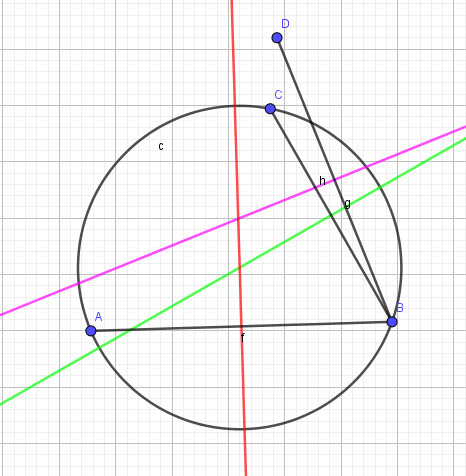
\includegraphics[width=5cm,height=5cm]{geometry/De.png} \newline \newline

现在B有两个备选出边BC和BD。其中$\angle ABC < \angle ABD$

如果D在ABC外接圆内,则BC边需要被立即删除。如果不在,则我们当前只需要考虑C点，而不需要考虑D点。

所以,只要维护一个点的所有出边的极角序,就可以快速查找。

现在我们需要支持的操作是：查询相邻点、插入、删除,把原本存边的邻接表改成双向链表就可以$O(1)$进行操作了。
\end{multicols}
\end{frame}

\begin{frame}{V图的定义}
定义$H(P_1,P_2)$为到$P_1$点比到$P_2$点距离近的点的集合。

对于平面上n个点的点集S,定义$V(P_i)=\bigcap_{i \neq j}H(P_i,P_j)$,即$V(P_i)$表示到$P_i$点的距离小于其他所有点的距离的点的集合,这显然是一个不多于$n-1$条边的凸多边形区域(有可能不闭合),称为关联与 $P_i$的Voronoi多边形或关联与$p_i$的Voronoi多边形域。

对于点集S中的每个点都可以做一个Voronoi多边形(域),这样n个Voronoi多边形(域)组成的图形叫做Voronoi图。
\end{frame}

\begin{frame}{V图的构造}
暴力构造法：对于每个点，求出所有的$H(P_i,P_j)$，然后对于$n-1$个半平面求交。$O(nlogn)$

Voronoi图与Delaunay三角剖分互为对偶图，所以可以先求出点集的Delaunay三角剖分，然后将图形对偶，这样就得到了Voronoi图。

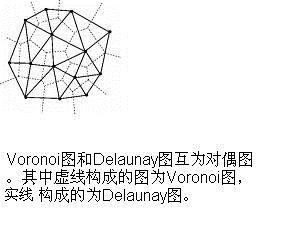
\includegraphics[height=5cm]{geometry/v.png}
\end{frame}

\begin{frame}{V图的构造}{对偶性证明}
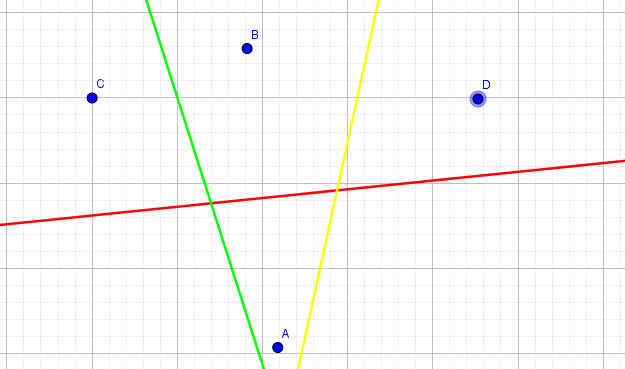
\includegraphics[height=4cm]{geometry/vgraph.png}

证明：在图中作出AB两个点的中垂线PQ，那么包含AB的圆一定在直线PQ上。
又由于圆P中不能包含其它点，对于任意点C满足P位于BC的中垂线的靠B一侧。

如果AB相连那么取红色直线中间夹的这一部分都是合法圆心。

如果AB不相连那么也不存在圆P。
\end{frame}

\begin{frame}
\frametitle{Delaunay三角剖分对偶得Voronoi图}
因为Voronoi点正好是三条Voronoi边的交点，也就是说Voronoi点是形成三边的三点的外接圆圆心。
那么对偶的方法就是：
\begin{enumerate}
    \item 先将每个Delaunay三角形的外接圆圆心求出。
    \item 如果两个三角形有公共边，那么在它们的外接圆圆心之间连一条边。
    \item 如果某一条Delaunay边在点集的凸包上，那么以这条边所在的三角形的外接圆圆心为起点，向该边做垂直射线。
\end{enumerate}

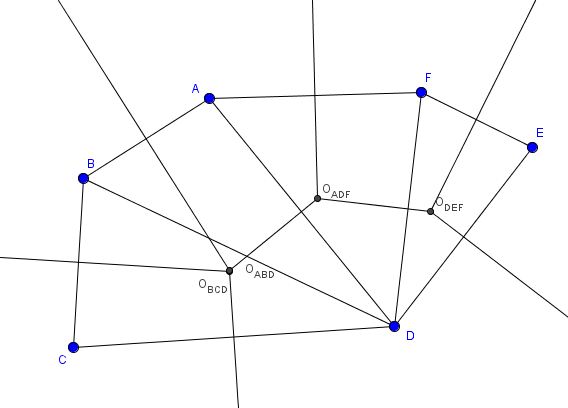
\includegraphics[height=3cm]{geometry/d.png}
\end{frame}

\begin{frame}
\frametitle{V图的应用}
\framesubtitle{平面MST问题}
\pause
给定平面上的一些点，要选择一些点对两两连边，两点之间的边长为欧几里得距离，求最小生成树。

\pause
结论：最小生成树上的边一定是Delaunay三角剖分中的边。

\pause
证明：根据Delaunay三角剖分的定义，如果ab之间没有边相连，则以ab为直径的圆中必然有其它点c。

而我们知道，圆内最大距离$=$直径，而ab就是直径，所以$|ac|,|bc| \le |ab|$

我们把边$(a,b)$删除，如果c在连通块a，则连接边$(c,b)$，否则连接边$(c,a)$，这样不会更差。

\pause
所以，构出三角剖分做最小生成树即可。复杂度$n(logn+\alpha(n))$
\end{frame}

\begin{frame}
\frametitle{V图的应用}
\pause
有一个$n*m$的矩形，矩形内有若干个点组成点集S。现在要把一个圆从矩形的左边平移到矩形的右边。要求圆不能和S中的点以及矩形边界相交。问圆的半径最大值。

\pause
问题实际上就是，找到一条路径，使得这条路径上的点到矩形边界和S中的点的最小距离最大。

\pause
经过分析可以发现，最优路线一定是沿V图中的边走。(如果偏离了V图中的边那么会使得到某个点的距离变小)

\pause
还要注意一个细节：可能是沿着边界走，所以我们对于所有点$(x,y)$都新建两个点$(x,0)$和$(x,m)$。

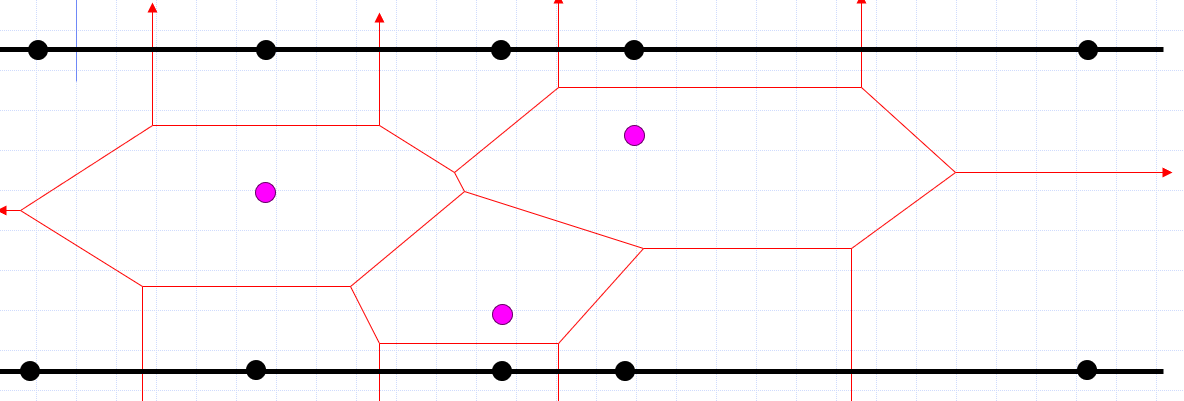
\includegraphics[height=2cm]{geometry/vgraph3.png}
\end{frame}
